%-----------------------------------------------------------------------------------------------------------------------------------------------%
%	The MIT License (MIT)
%
%	Copyright (c) 2021 Jitin Nair
%
%	Permission is hereby granted, free of charge, to any person obtaining a copy
%	of this software and associated documentation files (the "Software"), to deal
%	in the Software without restriction, including without limitation the rights
%	to use, copy, modify, merge, publish, distribute, sublicense, and/or sell
%	copies of the Software, and to permit persons to whom the Software is
%	furnished to do so, subject to the following conditions:
%	
%	THE SOFTWARE IS PROVIDED "AS IS", WITHOUT WARRANTY OF ANY KIND, EXPRESS OR
%	IMPLIED, INCLUDING BUT NOT LIMITED TO THE WARRANTIES OF MERCHANTABILITY,
%	FITNESS FOR A PARTICULAR PURPOSE AND NONINFRINGEMENT. IN NO EVENT SHALL THE
%	AUTHORS OR COPYRIGHT HOLDERS BE LIABLE FOR ANY CLAIM, DAMAGES OR OTHER
%	LIABILITY, WHETHER IN AN ACTION OF CONTRACT, TORT OR OTHERWISE, ARISING FROM,
%	OUT OF OR IN CONNECTION WITH THE SOFTWARE OR THE USE OR OTHER DEALINGS IN
%	THE SOFTWARE.
%	
%
%-----------------------------------------------------------------------------------------------------------------------------------------------%

%----------------------------------------------------------------------------------------
%	DOCUMENT DEFINITION
%----------------------------------------------------------------------------------------

% article class because we want to fully customize the page and not use a cv template
\documentclass[a4paper,12pt]{article}

%----------------------------------------------------------------------------------------
%	FONT
%----------------------------------------------------------------------------------------

% % fontspec allows you to use TTF/OTF fonts directly
% \usepackage{fontspec}
% \defaultfontfeatures{Ligatures=TeX}

% % modified for ShareLaTeX use
% \setmainfont[
% SmallCapsFont = Fontin-SmallCaps.otf,
% BoldFont = Fontin-Bold.otf,
% ItalicFont = Fontin-Italic.otf
% ]
% {Fontin.otf}

%----------------------------------------------------------------------------------------
%	PACKAGES
%----------------------------------------------------------------------------------------
\usepackage{url}
\usepackage{parskip} 	

%other packages for formatting
\RequirePackage{color}
\RequirePackage{graphicx}
\usepackage[usenames,dvipsnames]{xcolor}
\usepackage[scale=0.9]{geometry}

%tabularx environment
\usepackage{tabularx}

%for lists within experience section
\usepackage{enumitem}

% centered version of 'X' col. type
\newcolumntype{C}{>{\centering\arraybackslash}X} 

%to prevent spillover of tabular into next pages
\usepackage{supertabular}
\usepackage{tabularx}
\newlength{\fullcollw}
\setlength{\fullcollw}{0.47\textwidth}

%custom \section
\usepackage{titlesec}				
\usepackage{multicol}
\usepackage{multirow}

%CV Sections inspired by: 
%http://stefano.italians.nl/archives/26
\titleformat{\section}{\Large\scshape\raggedright}{}{0em}{}[\titlerule]
\titlespacing{\section}{0pt}{10pt}{10pt}

%for publications
\usepackage[style=authoryear,sorting=ynt, maxbibnames=2]{biblatex}

%Setup hyperref package, and colours for links
\usepackage[unicode, draft=false]{hyperref}
\definecolor{linkcolour}{rgb}{0,0.2,0.6}
\hypersetup{colorlinks,breaklinks,urlcolor=linkcolour,linkcolor=linkcolour}
\addbibresource{citations.bib}
\setlength\bibitemsep{1em}

%for social icons
\usepackage{fontawesome5}

%debug page outer frames
%\usepackage{showframe}

%----------------------------------------------------------------------------------------
%	BEGIN DOCUMENT
%----------------------------------------------------------------------------------------
\begin{document}

% non-numbered pages
\pagestyle{empty} 

%----------------------------------------------------------------------------------------
%	TITLE
%----------------------------------------------------------------------------------------

% \begin{tabularx}{\linewidth}{ @{}X X@{} }
% \huge{Your Name}\vspace{2pt} & \hfill \emoji{incoming-envelope} email@email.com \\
% \raisebox{-0.05\height}\faGithub\ username \ | \
% \raisebox{-0.00\height}\faLinkedin\ username \ | \ \raisebox{-0.05\height}\faGlobe \ mysite.com  & \hfill \emoji{calling} number
% \end{tabularx}
\begin{figure}[h]
	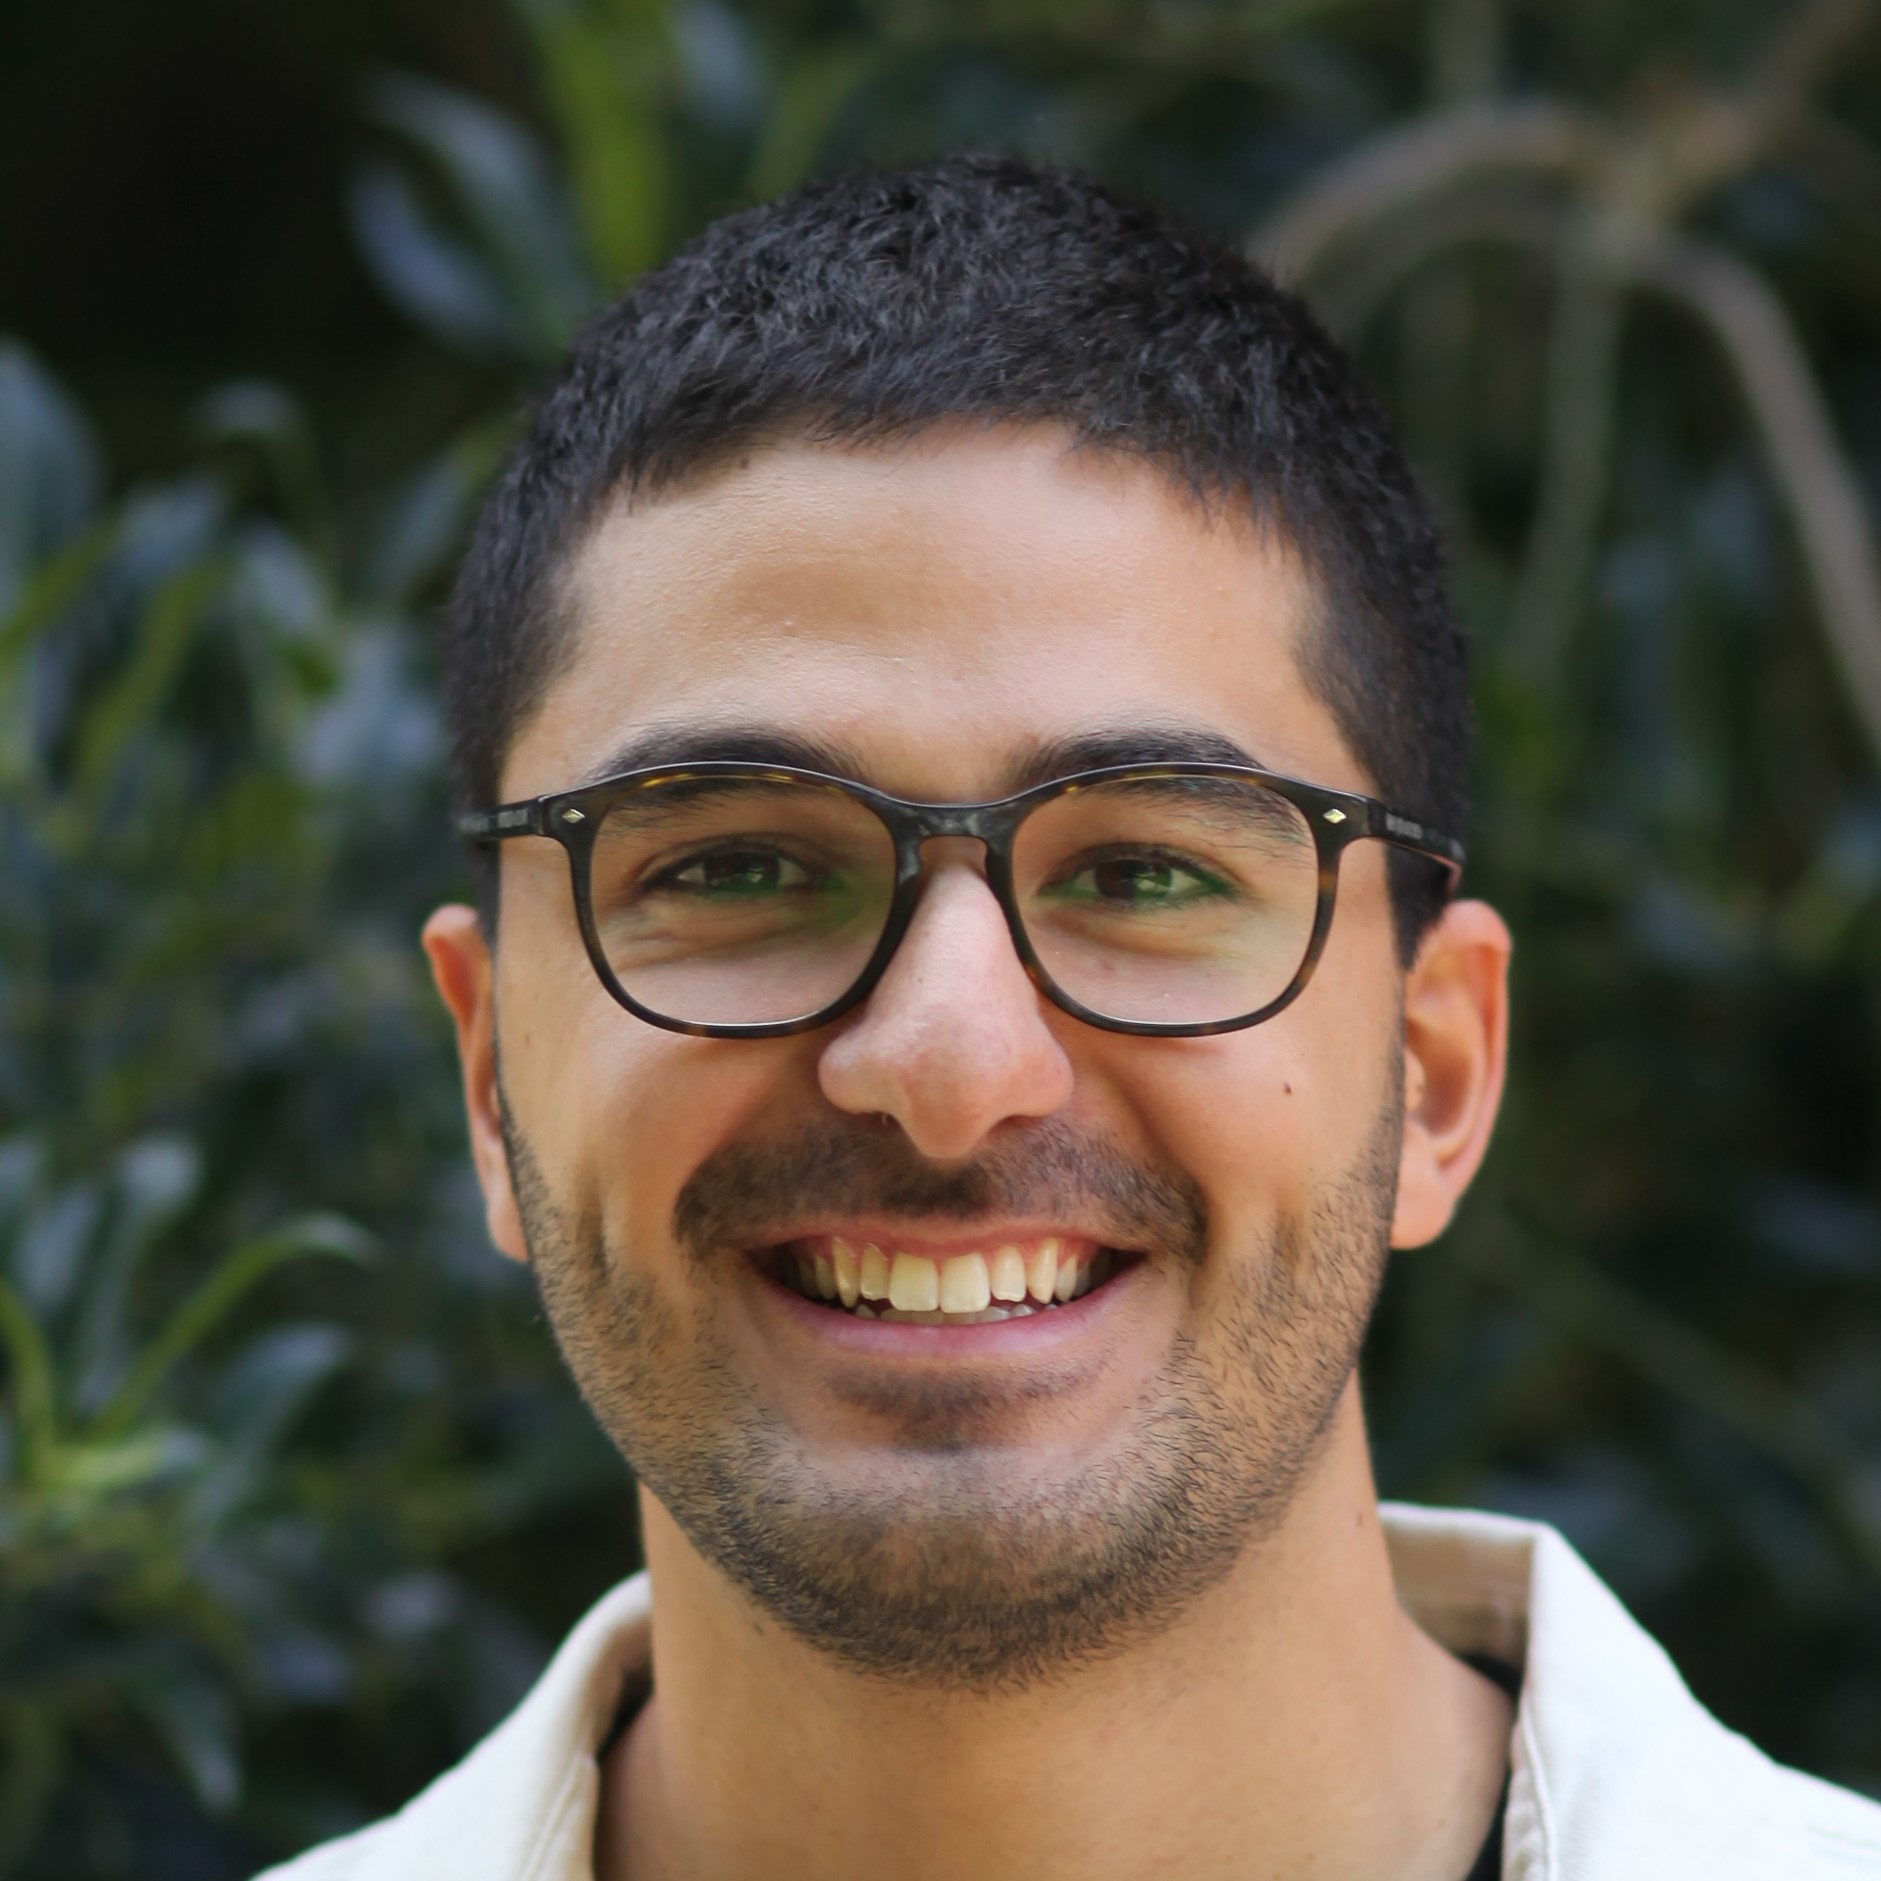
\includegraphics[width=2.8cm]{figures/bild_cv.jpg}
	\centering
\end{figure}
\begin{tabularx}{\linewidth}{@{} C @{}}
\Huge{Amin Alian} \\[7.5pt]

\href{https://github.com/aminager}{\raisebox{-0.05\height}\faGithub\ Aminager} \ $|$ \ 
\href{https://linkedin.com/in/aminalian}{\raisebox{-0.05\height}\faLinkedin\ Amin Alian} \ $|$ \ 
% \href{https://mysite.com}{\raisebox{-0.05\height}\faGlobe \ mysite.com} \ $|$ \ 
\href{mailto:alianamin00@gmail.com}{\raisebox{-0.05\height}\faEnvelope \ alianamin00@gmail.com} \ $|$ \ 
\href{tel:+46761927594}{\raisebox{-0.05\height}\faMobile \ +46 76 192 75 94} \\
\end{tabularx}

%----------------------------------------------------------------------------------------
% EXPERIENCE SECTIONS
%----------------------------------------------------------------------------------------

%Interests/ Keywords/ Summary
\section{Summary}
Hey! My name is Amin and I’m currently in my seventh semester at LTH,
studying Computer Science Engineering, specialising in Software. I’m
fluent in Swedish, English and Persian. Being around people gives me
energy, but my foremost quality is my calm. I relax by playing sports and
am looking forward to new and ambitious tasks.

%Experience
\section{Work Experience}

\begin{tabularx}{\linewidth}{ @{}l r@{} }
\textbf{Tetra Pak, Student Talent Programme} & \hfill Jun 2022 - present \\[3.75pt]
\multicolumn{2}{@{}X@{}}{I am a technical expert at Tetra Pak on the Microsoft Ecosystem, such as PowerApps, Power BI and Power Automate. I have created my own reports in Power BI which are used in the engineers daily work. In PowerApps I also developed apps by configuring a back-end and creating a front-end to reduce the time loss in their daily work.}  \\
\end{tabularx}

\begin{tabularx}{\linewidth}{ @{}l r@{} }
\textbf{DHL Express, Courier} & \hfill Jun 2021 - Aug 2021 \\[3.75pt]
\multicolumn{2}{@{}X@{}}{
    As a courier the daily tasks were very independent and individual. This meant that I had to use critical thinking and challenge myself to solve difficulties and problems that arose everyday. My biggest takeaway from the position was how much of a difference it makes to allow myself to ask questions. By collaborating and sharing knowledge we achieved more.
}
\end{tabularx}

%Projects
%\section{Projects}

%\begin{tabularx}{\linewidth}{ @{}l r@{} }
%\textbf{Some Project} & \hfill \href{https://some-link.com}{Link to Demo} \\[3.75pt]
%\multicolumn{2}{@{}X@{}}{long long line of blah blah that will wrap when the table fills the column width long long line of blah blah that will wrap when the table fills the column width long long line of blah blah that will wrap when the table fills the column width long long line of blah blah that will wrap when the table fills the column width}  \\
%\end{tabularx}

%----------------------------------------------------------------------------------------
%	EDUCATION
%----------------------------------------------------------------------------------------
\section{Education}
\begin{tabularx}{\linewidth}{@{}l X@{}}	
2019 - present (2024) & MSE Comp. Sci. at \textbf{Lund University, LTH} \hfill \normalsize (GPA: 3.3/4.0) \\

2016 - 2019 & Upper Secondary School at \textbf{Kungsholmens Gymnasium} \hfill (GPA: 20.8/22.5) \\ 
\end{tabularx}

%----------------------------------------------------------------------------------------
%	PUBLICATIONS
%----------------------------------------------------------------------------------------
\section{Voluntary Work}
\begin{tabularx}{\linewidth}{ @{}l r@{} }
\textbf{Vice Chairman of the Activity Committee, Comp
Sci Guild LTH} & \hfill Jan 2020 - Dec 2020 \\[3.75pt]
\multicolumn{2}{@{}X@{}}{
    As the Vice Chairman I arranged and executed events together with other
    guilds at LTH. I was ultimately in charge of organisation of events and
    integration in the guild.
}
\end{tabularx}

\begin{tabularx}{\linewidth}{ @{}l r@{} }
\textbf{Web master, Student Union at Kungsholmens
Gymnasium} & \hfill Mar 2018 - Mar 2019 \\[3.75pt]
\multicolumn{2}{@{}X@{}}{
    I was in charge of making sure the website was maintained, developed and secure
}
\end{tabularx}

%----------------------------------------------------------------------------------------
%	SKILLS
%----------------------------------------------------------------------------------------
\section{Skills}
\begin{tabularx}{\linewidth}{@{}l X@{}}
Programming &  \normalsize{I am very comfortable with programming and approaching new tasks. I have university experience in working with Scrum, Agile and team development. I am most comfortable in Python and Java, but I am eager to learn more. I have worked in Scala, React as well as PowerQuery and DAX as well.}\\
\end{tabularx}

\vfill
\center{\footnotesize Last updated: \today}

\end{document}
